\setcounter{equation}{0}
\setcounter{figure}{0}

\section{Electromagnetic Plane Waves}

Name \rule{2.0in}{0.1pt}\hfill{}Section \rule{1.0in}{0.1pt}\hfill{}Date
\rule{1.0in}{0.1pt}

\textbf{Objective:} 

To investigate electromagnetic waves, using two different software simulations.

%\begin{itemize}
%\item The effect of changing magnetic fields on induced emf and current.
%\end{itemize}


\textbf{Activity 1: Simulating Electromagnetic Waves}

\begin{enumerate}

\item Open {\it Internet Explorer} ({\it IE$~$}) and go to the website
{\tt \verb!http://www.falstad.com/emwave2!}. A Java applet will pop up showing
brightly colored waves like the ones in Figure 1 propagating outward. 
%from our oscillating electric dipole. 
If you don't see this window, consult your instructor.
\begin{figure}[hbt]
\begin{center}
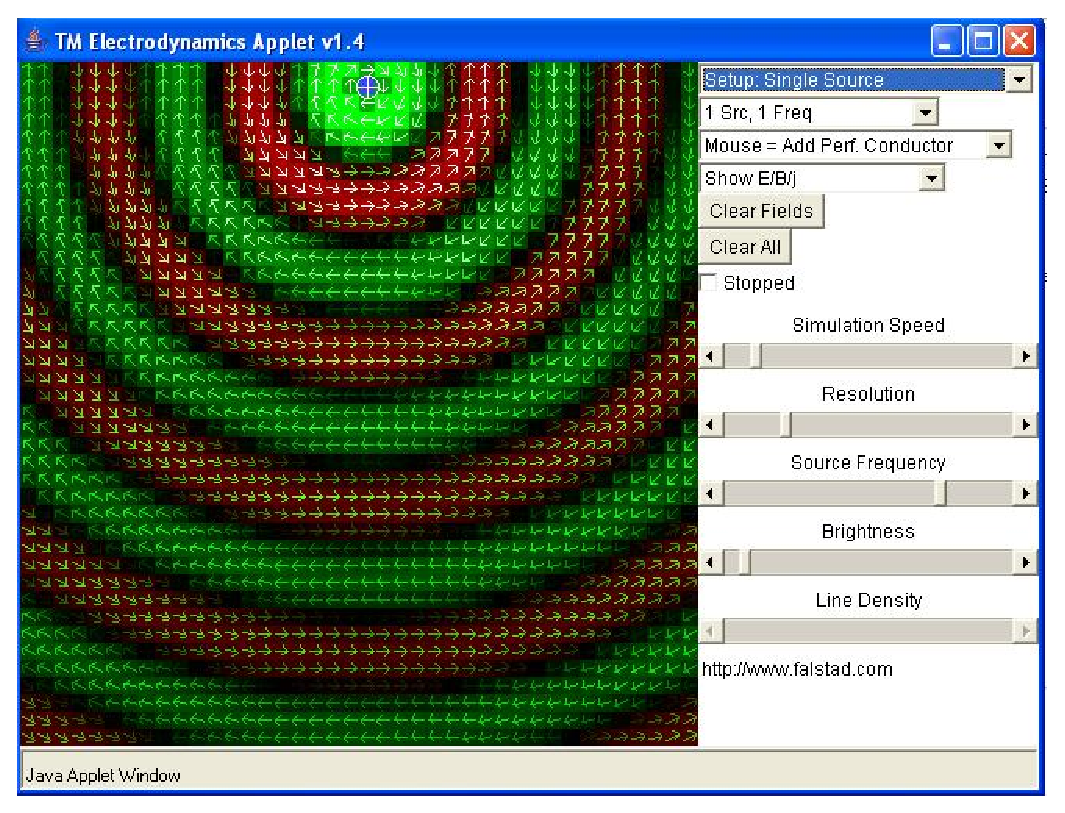
\includegraphics[width=6.0in]{plane_waves/emwaves1.eps}
\caption{Applet showing electromagnetic waves.}
\end{center}
\end{figure}

\item It is useful to slow down the simulation speed to observe the waves more clearly.
Do this using the slide labeled
{\tt Simulation Speed} on the right-hand side of the applet window.

\item What you see is an ``oscillating dipole'', very similar to the generation of radio waves with an antenna.
Charges (usually electrons) are driven up and down in the antenna and emit electromagnetic 
waves.  
The alternating yellow and blue circle at the top of the applet is the source (the dipole)
as viewed from above.  Any yellow in the simulation indicates electrical current (charge) moving towards you, and any blue indicates current away from you.  Does the simulation show any current (motion of charges) flowing far away from the source?
\vspace{1.5cm}

\item The green and red colors indicate the electric field; green areas are positive 
($\vec E$ toward you) and red areas are negative ($\vec E$ away from you). 
The electric field is always perpendicular to the plane of the screen.
In addition to the colors, arrows indicate the 
direction of the magnetic field, which is always in the plane of the screen.  

What direction does the electric field point when the magnetic field is to the right?
\vspace{1cm}

What direction does the electric field point when the magnetic field is to the left?
\vspace{1cm}

\item Are the electric and magnetic fields always perperndicular to each other?
\vspace{1.0cm}

%\item Go back to your predictions in Activity 2 about the directions of the $\vec E$ 
%and $\vec B$ fields.
%Compare your predictions with these observations. Correct any disagreements.
%\vspace{2.0cm}

\item If you made predictions in Activity 2 of the first induction lab about the directions of the $\vec E$ 
and $\vec B$ fields, compare those predictions with your observations here. Correct any disagreements.
\vspace{2.0cm}

\item When you drop a pebble in a pond of water, the waves go out in circles. The shape of the wave ``front'', which is what you get when you connect all the points on the crest of a single wave, is a circle.   In this simulation, the waves are radiating out in three dimensions, not two.  In this three-dimensional case, what is the shape of the wave fronts near the source?
\vspace{1cm}

Far away from the pebble in the pond, the circular wave fronts hitting the shore look like straight lines because at a small length scale you don't notice their slight curvature. In the three-dimensional case in the simulation, what is the apparent shape of a wave front far away from the source, if you ignore the slight curvature?
\vspace{1cm}


\item Reduce the frequency of the oscillation of the dipole using the slide labeled
{\tt Source Frequency} on the right-hand side of the applet.
You may have to increase the brightness of the applet using the slide labeled
{\tt Brightness}.
What happens to the distance between successive peaks or crests of the waves defined by the red regions in the
applet)?
This distance is called the wavelength and it is characteristic of a particular
wave.
Light, for example,  is an electromagnetic wave and different wavelengths correspond 
to different colors.
\vspace{2.0cm}

%\item One can calculate a quantity known as the Poynting vector which points in the direction of the flow of energy in an %individual wave. Make the applet draw the Poynting vector by clicking on the arrow in the box with 
%{\tt Show E/B/j} entered in it. Scroll up or down until you find
%{\tt Show Poynting vector} and highlight it.
%In what direction does the energy flow?
%\vspace{1.0cm}

\item The ``Poynting vector'' is defined to point in the direction of the flow of energy in a wave. Its direction is given by $\vec E \times \vec B$.  What is the direction of $\vec E \times \vec B$ where the color of the wave is red?
\vspace{1.0cm}

What is the direction of $\vec E \times \vec B$ where the color of the wave is green?
\vspace{1.0cm}

Make the applet draw the Poynting vector by clicking on the arrow in the box with 
{\tt Show E/B/j} entered in it. Scroll up or down until you find
{\tt Show Poynting vector} and highlight it.
In what direction does the energy flow?  (Does that agree with what you just said about $\vec E \times \vec B$?)
\vspace{1.0cm}

\item Go back to {\tt Show E/B/j} mode you were in before. 
Just for fun, we want to introduce one of the central phenomena associated
with waves known as interference.
Go to the second menu from the top of the right-hand side of the applet.
Click and highlight {\tt 2 Src, 1 Freq}.
This will place an additional oscillating dipole at the bottom of the applet.
Describe what happens.
When waves add together they can cancel one another (this is called destructive 
interference).
Do you observe destructive interference?
What do you think happens for constructive interference?
\vspace{1.5cm}

\item Now use your mouse to grab one of the sources and drag it to a position
near the other one.
How does the interference pattern change?
Try different positions for the source (move it closer or further away).
Describe what you see.
If these were light waves, where would you see bright light?
Where would you see dark regions?
\vspace{2.0cm}

\end{enumerate}

\textbf{Activity 2: Plane Waves}

%You just completed a study of spherical waves emitted by a dipole source.
%We now want to consider another type of wave that we will study when we explore light.

\begin{enumerate}

\item  Use {\it IE} to go to the site
{\tt \verb!http://www.amanogawa.com/archive/PlaneWave/PlaneWave-2.html!} and a Java applet will appear 
like the one in Figure 2. 
If you don't see this window, consult your instructor.
The top panel of the applet shows an electromagnetic plane wave.
The red lines represent the direction and magnitude of the $\vec E$ field and the
blue ones do the same for the $\vec B$ field.
NOTE: The magnetic field in this applet is labeled $\vec H$.
In this case, this is exactly the same as our previous $\vec B$.
To eliminate some unnecessary lines, click the box beside {\tt Phasors} so the check in the box 
disappears.
\begin{figure}[hbt]
\begin{center}
%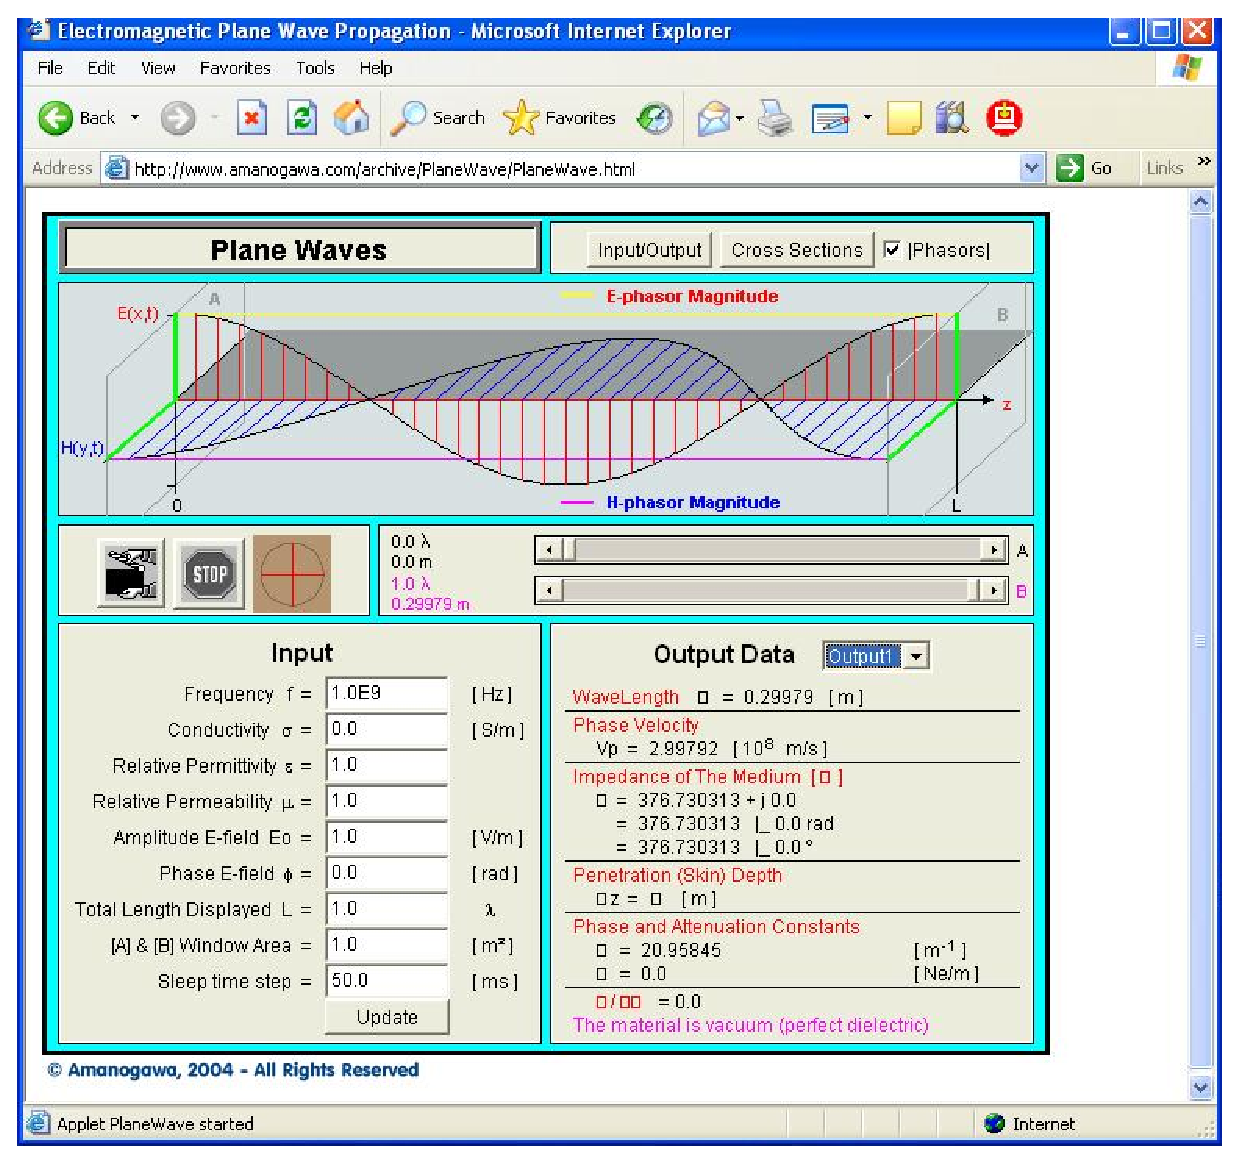
\includegraphics[width=4.0in]{plane_waves/emwaves3.eps}
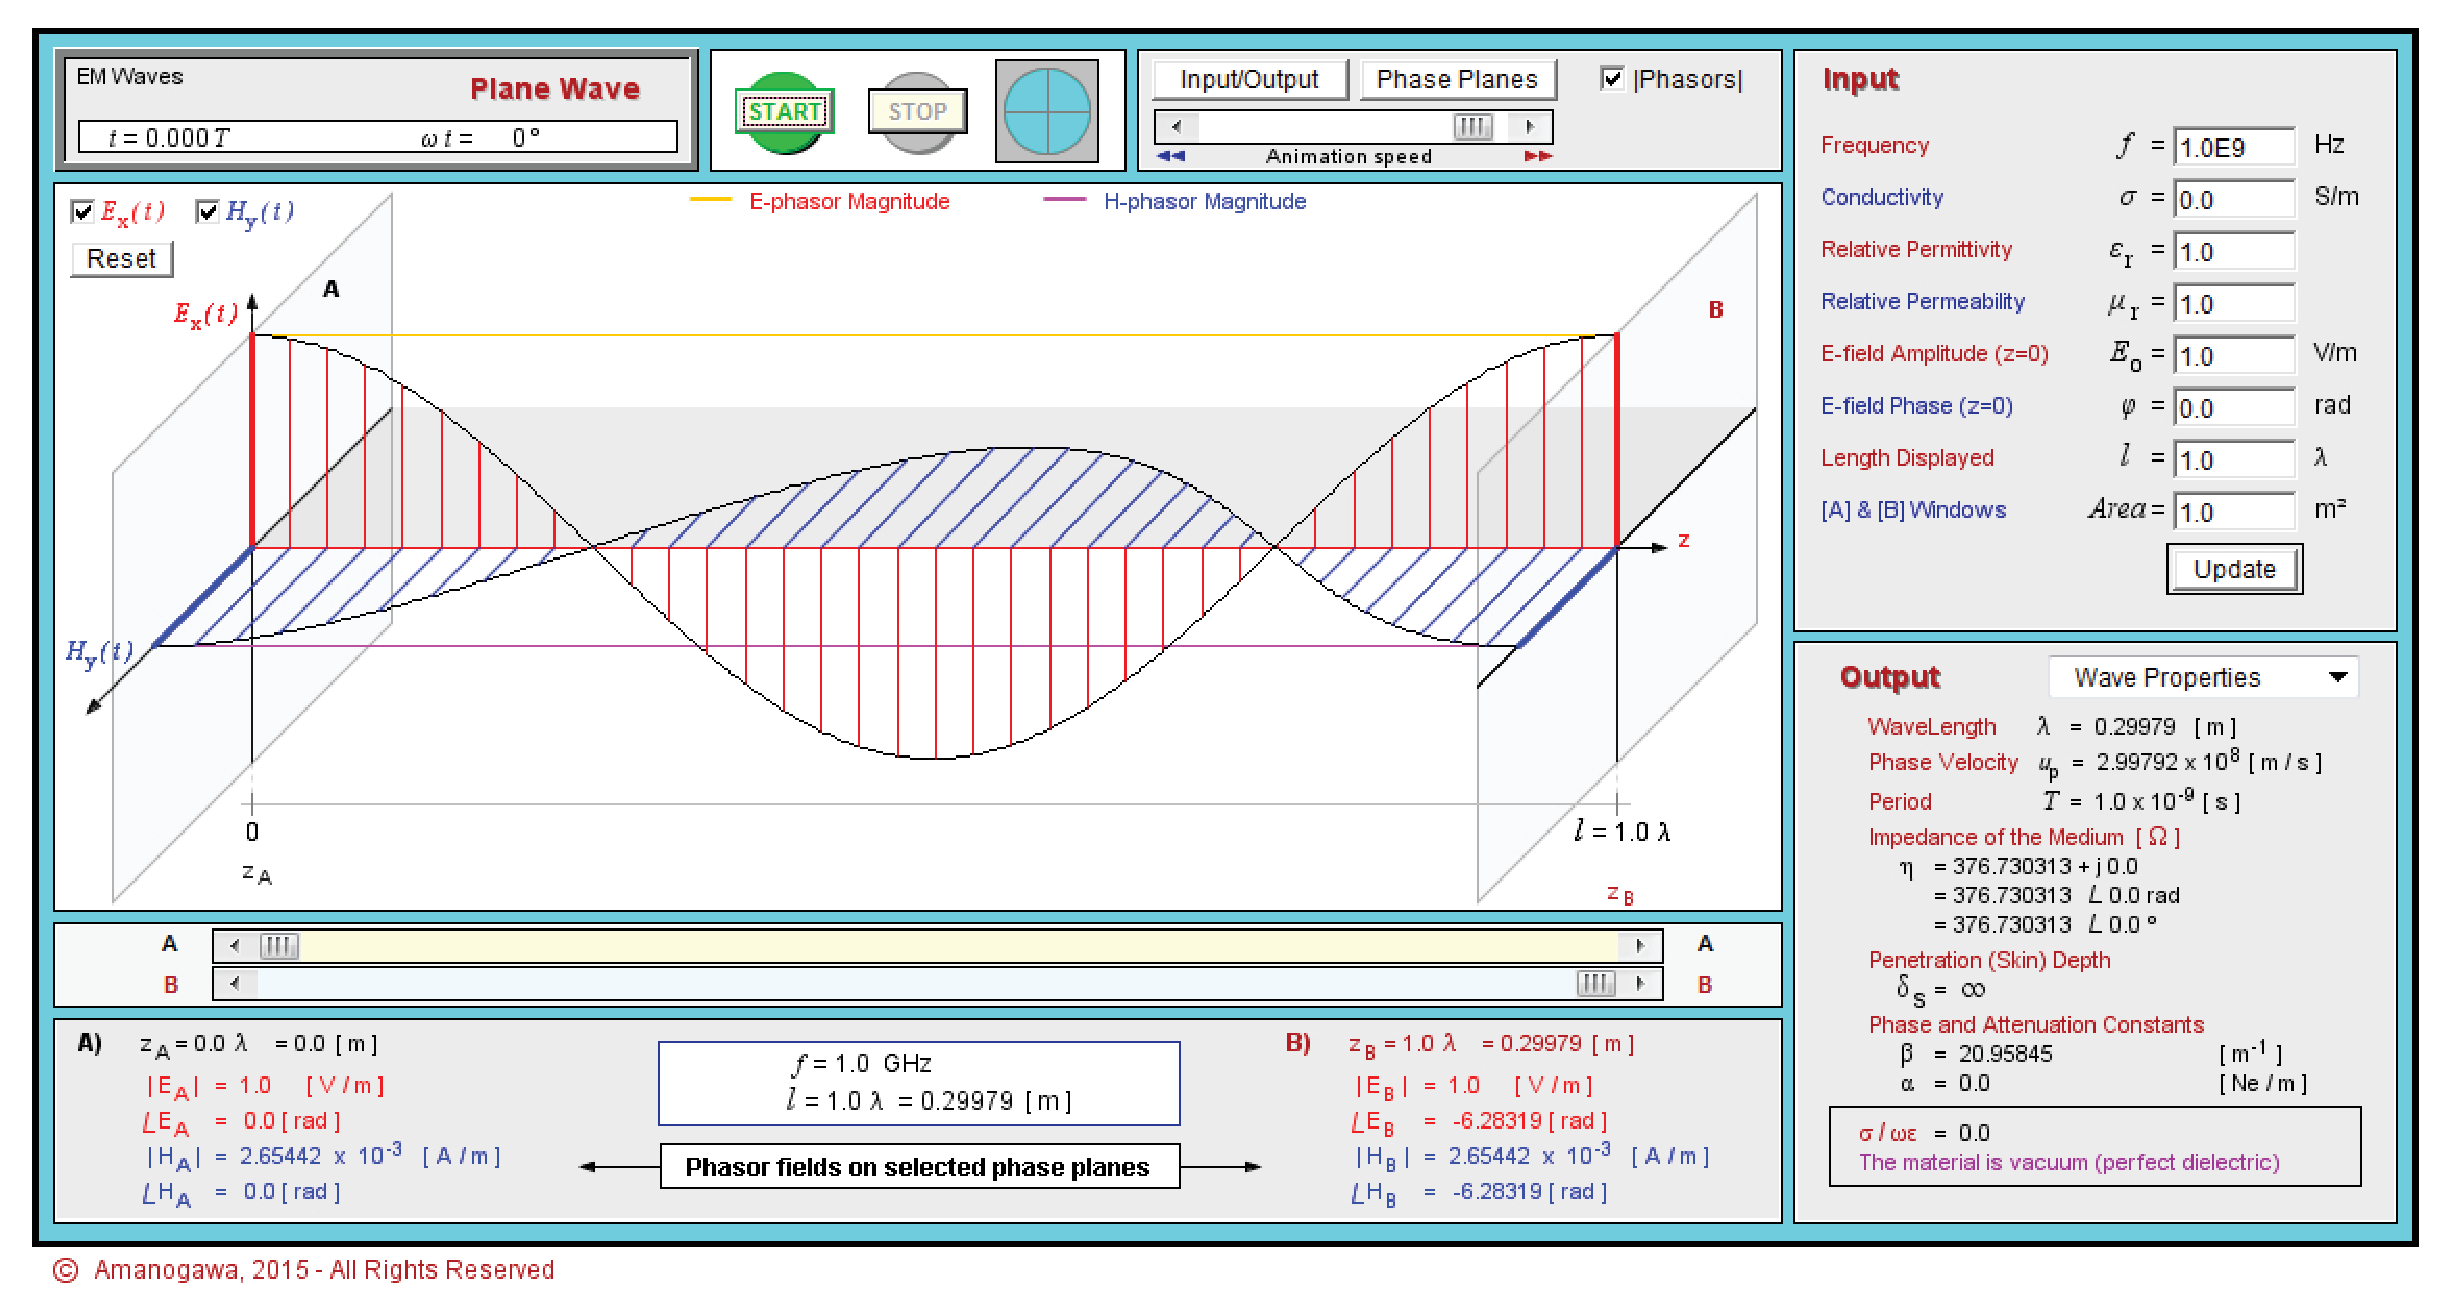
\includegraphics[width=5.0in]{plane_waves/plane_wave_screenshot.eps}
\caption{Applet showing plane electromagnetic waves.}
\end{center}
\end{figure}

\item Click the start button to watch the wave move or propagate. The button is the one to the left of the STOP button on the top of the applet.
Describe what happens to the electric and magnetic fields and how they are related
({\it i.e.} When the $\vec E$ is large, what is the $\vec B$ field doing?).
\vspace{3.0cm}

\item What is the orientation of the $\vec E$ field?
What is the orientation of the $\vec B$ field?
Does $\vec E \times \vec B$ point in the direction of energy flow, as it did in the previous activity?
\vspace{2.0cm}

%\item Why do you think it's called a plane wave?
%\vspace{2.0cm}

\item Click on the {\tt Phase Planes} button at the top of the applet.
You will see new panels that show the $\vec E$ (red) and $\vec B$ (blue) vectors in cross section at the
planes $A$ and $B$ labeled in the top panel.
Use these vectors to confirm your observations in parts 2.2-2.3, above.
\vspace{3.0cm}

\item Use the $B$ slide at the bottom of the applet to move the $B$ cross 
section position.
Set it one-half wavelength from the $A$ cross section.
How are the $\vec E$ and $\vec B$ vectors in the $A$ cross section related to their partners 
in the $B$ cross section.
What will be the total electric and magnetic fields if two waves are added that are out of line
by one-half wavelength?
\vspace{1.5cm}

\item The electromagnetic wave in this simulation is called a ``plane wave'' because its wavefronts are shaped like planes.  What is the orientation of these planes?  (Perpendicular to $\vec E$?  Perpendicular to the $z$ axis? Something else?) 
\vspace{1.5cm}

\item Stop the simulation and slide the $B$ phase plane to a spot where the electric field is a maximum (the crest of a wave).  The phase plane is explicitely showing you the values of $\vec E$ and $\vec B$ at that one point on the wave front, located on the $z$ axis.  If you moved from that point in the positive $x$ direction, would $\vec E$ increase, decrease, or stay the same?  Would $\vec B$ increase, decrease, or stay the same? 
\vspace{2.0cm}

\end{enumerate}

\textbf{Activity 3}

An electromagnetic \textbf{PLANE} wave is described by
\begin{align*}
\vec E &= E_{MAX} \cos \left ( kx - \omega t \right ) \hat x\\
\vec B &= B_{MAX} \cos \left ( kx - \omega t \right ) \hat y,
\end{align*}
and has a wavelength of $\lambda =12$ meters.  All $(x,y,z)$ points in this activity are in meters.
\vspace{0.1in}

\begin{enumerate}

\item Draw a sketch of the wave on the axes below, at time $t=0$.
\begin{center}
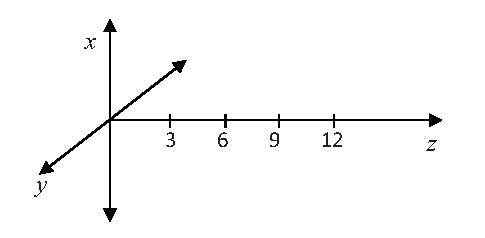
\includegraphics[width=0.4\textwidth]{plane_waves/em_waves_axes.eps}
\end{center}

\item At $t=0$, find both $\vec E$ and $\vec B$ at the points $(0,0,0), (0,0,3), (0,0,6),$ and $(0,0,9)$.  (Your answers are vectors, and should include both \textbf{magnitude} and \textbf{direction}.) 
\vspace{1.0in}

\item At $t=0$, find both $\vec E$ and $\vec B$ at the points $(0,1,0), (1,0,0), (1,1,0),$ and $(1,1,3)$.  (Remember, it's a \textbf{PLANE} wave….)
\vspace{1.0in}

\item Find the period $T$ and frequency $f$ of the wave.  (Numerical answers, please.)
\vspace{1.0in}

\item At $t=10$ nsec, find $\vec E$ and $\vec B$ at the points $(0,0,0), (0,0,3), (0,0,6), (0,0,9),$ and $(1,2,3)$.  
\vspace{1.0in}
\end{enumerate}


